\documentclass[]{article}
\usepackage[pdftex]{graphicx}
\usepackage[top=1in, bottom=1in, right=1.25in, left=1.25in]{geometry}
\usepackage{hyperref}
\hypersetup{colorlinks=true, linkcolor=blue, urlcolor=blue}

\begin{document}
	\tableofcontents
	\newpage
	
	% Eigth Entry
	\section{Classwork on Brainstorming, etc 10/11/2012}
		\subsection{Stages in the Feasibility Stage}
			There are 5 stages in the next  portion of our development process:
			\begin{itemize}
				\item Stage 1: Brainstrom
				\item Stage 2: Identify Risk
				\item Stage 3: Prioritize Risks
				\item Stage 4: Develop Deliverables for each Risk
				\item Stage 5: Divide and Schedule work
			\end{itemize}
			
			\subsection{Brainstorming}
			There are three major sections to our project:
				\begin{itemize}
					\item Capturing
					\begin{itemize}
						\item All tasks related to capturing all information written on the whiteboard
					\end{itemize}
					\item Sending
					\begin{itemize}
						\item All tasks related to sending and recieving information between devices
					\end{itemize}
					\item Processing
					\begin{itemize}
						\item All tasks related to processing the images once they are recieved by the linux machine
					\end{itemize}
				\end{itemize}
			
			\emph{Capturing} 
			\begin{itemize}
				\item Decide on a camera
				\item Designing/purchasing a stand
				\item Figure out setup stuff
				\item Determin min/max distance from board based on camera lense and number of megapixels
				\item Look into rooting camera (maybe. depends if it can install apps that aren't in the app store)
				\item Look into making image capturing process automated
				\item look into designing android app
				\item how to take periodic images
				\item how to communicate with camera using button or sensor
				\item adjust shutter speed and/or ISO to accomodate different light levels. (automatic with flash disabled)
			\end{itemize} 
			
			\emph{Sending}
			\begin{itemize}
				\item Look into communication between android and linux
				\item Ways to store/send images
				\item Ways to make sending info reliable
				\item How to send data automatically
				\item How to recieve data on linux
				\item How to automate linux processes
				\item How to send to/connect to moodle folder.
			\end{itemize}
			
			\emph{Processing}
			\begin{itemize}
				\item How to remove background noise
				\item how to stitch in information covered by professor
				\item how to change brightness/contrast
				\item look into better ways of processing images
				\item look into what image processing libraries are available
				\item maybe look into what programs are available to do these sorts of things for us.
				\item look into ways to automate actions performed by random programs
				\item look into ways to do what we want with premade programs and just automate the processes somehow
				\item What sorts of processing technologies are available to us?
			\end{itemize}
			
		\subsection{Identify Risks}
		There are are 3 main areas that represent the highest risks to our project:
			\begin{itemize}
				\item Image Proessing on the linux system
				\begin{itemize}
					\item Everything associated with it. How will we do this???
				\end{itemize}
				\item Deciding on Camera
				\begin{itemize}
					\item This will define how we will research the image captureing process. There isn't very much that we can do on the capturing side of things before this decision is made.
				\end{itemize}
				\item Look into how to use camera using application
				\begin{itemize}
					\item The creation of an application that will automate the image capturing process on the android camera
				\end{itemize}
			\end{itemize}
		\subsection{Deliverables}
			\emph{Deliverables for Processing:}
			\begin{itemize}
				\item Demo code that removes noise
				\item Demo code identifying professor on image
				\item Demo code removing professor from image
				\item Demo code splicing prof-free images together
				\item Demo code auto-grabbing new images + removing prof, splicing together, etc.
				\item Demo code of auto-everything
			\end{itemize}
			\emph{Deliverables for Capturing}
			\begin{itemize}
				\item Demo image taken by android camera by our own app
				\item Demo android camera taking pictures automatically every few seconds
				\item Demo app setup process such that it can be left to auto=take pictures all period
				\item Demo app sending photos to linux machine
				\item Auto=focus
				\item Manual Zoom during setup.
			\end{itemize}
		
	% Seventh Entry
	\section{Group Work With Colin To Finish Up Documentation 10/10/2012}
		\noindent \emph{Electronic Whiteboards-} \\
Smartboards are full sized, touch sensitive whiteboards. You can project images onto them with a projector and then make edits/additions to them with any pointed object. The touch sensitive board senses where you are writing on the board and adds electronic corrections to the image/document. These devices do not compete as directly with our project as the smartphone apps and the scanners because they are not nearly as portable. They are the size of a standard whiteboard and thus cannot be easily moved between classrooms.
            \begin{itemize}
                \item SMART Board
                \item Panasonic's Panaboard
                \item Hitachi's Starboard
                \item The Promethean Board
            \end{itemize}
			

			\subsection{Introduction}
The following paragraphs are descriptions of several smartphone apps that contain features wish to emulate in our own project. They in many ways solve the needs of our current clients. We therefore hope to take some of these phone-app features and modify them to better meet the needs of our own clients. \\
				\subsection*{Whiteboard Capture Pro}
Source: Beetlebug Software's website\\
{\color{red} \url{http://www.beetlebugsoftware.com/}} \\
					
This is an iPhone app that takes a picture of a white board and then analyzes it for key content. The user selects objects to remove from the photograph. This leaves only the writing on the board behind. The App then analyzes the writing and removes the background image of the whiteboard itself. This sometimes leaves fuzz or imperfections in the white background, so there is then a slider available to filter out this extra noise/fuzz that shows up in the end product. The resulting image is a pure white background with handwriting on it.These photos can then be saved, cropped, shared, and organized within-app tools. \\
				\subsection*{WBConference}
Source: Elecom'e website\\
{\color{red} \url{http://app.elecom.co.jp/en/wbcap/ios/manual.html}} \\
					
This is an Android app that competes with our product because it is another whiteboard capturing device. WBConference differs from Whiteboard Capture Pro in that it is able to automatically recognize which sections of the board are whiteboard. This then allows it to apply its ìmagnified keystone correctionî to remove the excess background imagery. In cases that it cannot recognize the board you can zoom in on just the board boundaries manually before capturing the image. The app has contrast adjustment and image rotation as well so you can take images from any orientation without problems.This app has editing features as well so you can add postscripts or speech bubbles to the images. The files can then be saved as PDFs along with any notes you want to add to them.This app has a widget for the home screen for quick image capturing, and you can set up an email address for quick delivery of the images to an external source. \\
				\subsection{CamScanner -Phone PDF Creator}
Source: Intsig's Website
{\color{red} \url{http://www.intsig.com/en/camscanner.html}} \\
					
This is the most downloaded ëscannerí app on the market. With it you can take photos of any document, whiteboard, etc that you want. You then go through an editing process in which you can select the important portion of the photograph, change the detail level, contrast, light/darkness etc. It will then save your new document in any number of saved folders. You can make notes about each image and these notes will be saved with the image. You can email, print, fax, or transfer via Bluetooth any of the photos. You can also upload your images to google docs, evernote, skydrive, dropbox, or box.net. These documents get saved as PDFs. There are different enhancement modes: No enhance, low and high enhance, gray mode, and B\&W Document modes. These different modes will be better depending on the environment or object that youíre trying to scan. The B\&W mode is particularly helpful when scanning books/papers because it does a better job of removing the background noise. This app allows for batch photo taking and batch photo scanning, so you can take multiple pictures and it will scan them all at the same time. \\
				\subsection{Whiteboard Capture Pro}
Source: Magnicode's website\\
{\color{red} \url{http://www.magnicode.com/}} \\
					
This app is a dumbed down version of the previous three. It does the job, it scans and enhances images, it just isnít as well known as the others and thus doesnít have the money/time to invest in extra features. This aside, it does work, it is free, and it does save images as PDFs for later use. You can email these photos to yourself and store them in different photos. You can attach notes to your images and you can enhance the quality of the whiteboard picture with their auto-enhance tool. On the upside, it IS a much smaller program than your avg whiteboard capture app. Over all a smaller lighter free alternative. I installed this app on my phone and I had trouble using it because it kept crashing. \\

     \subsection*{Conclusion}
These smart phone apps will be some of the greatest competition to our project because they meet many of our client's needs already. Not only that, they're free applications so our clients wouldnt need to spend money either. The following is a list of features that we should attempt to emulate when designing our own product.

All of these applications contain ways to filter out background noise so that whiteboards appear pure white and text looks crisp and clean. This will be an important aspect of our own product because our image capture device will be subject to a wide variety of lighting situations and will need to be able to adapt to any of them.
Another key feature is the ability of these apps to save and send the images via email, google docs, and other online mediums. This will be an important point in our project as well.
Another good feature was the ability for some of the apps (CamScanner for example) to correct for image angles. If the board is photographed from an angle, the smartphone apps will compensate so that the final scanned image looks like it was taken straight on. \\

        \emph{Desirable features not found in smartphone apps:}
        \begin{itemize} \itemsep -2pt
            \item Photo splicing: These apps do not combine images to add in details covered by professor's body.
            \item Automatic: These apps do not automatically capture images, process them, and then send them away. They instead require user feedback every step of the way.
        \end{itemize}

By adding these features to the functionality currently found in modern apps we hope to create value for our customer.


	 \subsection*{Cameras we could use in our project}
Here are the current top three cameras that we think could help us the most when building our image capturing system.

\begin{itemize}
    \item Nikon COOLPIX S800c 16 MP Digital Camera
    \begin{itemize}
        \item \url{http://www.amazon.com/Nikon-COOLPIX-Digital-Optical-3-5-inch/dp/B0090SLKUM}
    \end{itemize}
    \item Samsung Camera EK-GC100 Galaxy Camera
    \begin{itemize}
        \item \url{http://pdadb.net/index.php?m=specs&id=3813&c=samsung_ek-gc100_galaxy_camera}
    \end{itemize}
    \item Polaroid SC1630 Smart Camera
    \begin{itemize}
        \item \url{http://www.upi.com/Science_News/2012/01/16/Polaroid-joins-digital-camera-arena/UPI-61851326750025/}
    \end{itemize}
\end{itemize}

We are interested in them because they are cameras running the Android operating system. This means that we could create our own custom application for these devices, greatly simplifying our design process. These cameras would also be useful because they can connect to Bucknell's wifi network. This would allow us to wirelessly transferr information from the cameras to whatever image processing hardware we decide to connect it to. The main drawbacks at the moment with these Android cameras is that two of them haven't been released yet (Samsung and Polaroid). IF they are released in time, they would be the most desireable of the various camera options available.

\subsection*{Details on Learning Disabilaties}
        \subsubsection*{Introduction}
One of the major motivating factors behind designing our image capturing system is to help meet the needs of students with disabilities. The term "students with disabilities" is a very broad term, however, so we would like to use the following section to help discribe some of the things that mildly disabled students have trouble with at Bucknell, and would therefore need our system to capture information presented on the board for them.
\\
Source: \\
{\color{red} \url{http://www.sfasu.edu/disabilityservices/facultyandstaff/for_service_providers/note_q_a.asp}} \\
\\
Disabilities that students might have that impair their ability to take notes:
    \begin{itemize}
        \item Visual Impairments
        \begin{itemize}
            \item May be fully blind and need notes translated into Braille
            \item May not see well and need large print letters
            \item May have trouble copying information from whiteboards, projectors, etc.
            \item May have trouble seeing certain colors when framed by a white or black background
        \end{itemize}
        \item Specific Learning Disabilities
        \begin{itemize}
            \item Reading Disability
            \item Writing Disability
            \item Spelling Disability
            \item Inability to copy what they see
            \item Inability to write what they hear
            \item Inability to write legibly
            \item Number Reversal problems
        \end{itemize}
        \item Mobility Impairments
        \begin{itemize}
            \item Physically unable to write
            \item Physically unable to write quickly
            \item May be unable to effectively handle a writing impliment
        \end{itemize}
        \item Partial or Full loss of hearing
    \end{itemize}

This is just a small portion of the many disabilities faced by students in universities around the world. We hope to help them by giving them full access all information presented on boards during lectures. By providing easily accessible, easily modifiable images, we hope to help even the playing field for students with disabilites.
Secondary goals of our project will help to make the learning process even easier. Some students get distracted if they see more than one line of text at a time. If we have enough time we will help these students by providing slide bars that will cover portions of the images that students are not currently viewing. This and many other minor features are things that we will accomplish if we have free time after completing our primary objectives.








	% Eigth Entry
	\section{Notes from Client meeting 10/05/2012}
	Point to git repository on website or it 'never happened.' The only things Thompson knows about are those found on the website.
	
	How image processing is generally don
	Types of image processing
	
	\emph{Important points given during meeting:}
		\begin{itemize}
			\item Wireless
			\item Way to tell system that "this" is a key fram/moment.
			\begin{itemize}
				\item Instructor marked key moments/frames with a button or gesture or something.
			\end{itemize}
			\item Generate list of 'it would be nice if...'
			\item Email about sitelines, optimal viewing angles, aspect ratios, etc.
			\item Re-organize Related Technologies
			\item Want: What are we DOING with all information presented in research/documentation
			\item Want: Paragraph at end of smartphone app summaries, synthasizing/analyzing information presented in summaries
			\item Microsoft: This project was very close to what we are going to do, that is why we are going into so much depth on it.
			\item Give information on the whole field of Image processing.
			\item Give information about students with various disabilities that would benefit from our product
			\begin{itemize}
				\item 'This is what the students need and why'
			\end{itemize}
		\end{itemize}
	\emph{Notes on stuff we'll be doing next:}
		\begin{itemize}
			\item Figure out what you're doing in the next couple months
			\item Look at what tasks you could be doing, analyze the risk of each task.
			\item Arrange everything by risk. Highest risk on top!
			\item Assign people reduce the risks of each task
			\begin{itemize}
				\item You can have multiple people working on a single thing. The idea is to reduce the high risk tasks asap so that they don't kill the project later on.
			\end{itemize}
			\item Assign 3-4 deliverable items to each person to reduce risk
			\item Can have multiple people per task
			\item Throw resources at the rediculously risky to get it done, else project fails
		\end{itemize}
	% Seventh Entry
	\section{Group work on Memo 10/03/2012}
		Worked with Colin and Phil to create the memo for our 10/05/12 meeting.


	% Sixth Entry
	\section{Individual Work on Further Research on Phone Apps 09/20/2012}
	
		\subsection{APPS}
		I was looking into android cameras earlier and found two possible candidates. One of them (The Nikon) has been released already, but the Samsung looks like a much better product if we can get it in time.
		
		Nikon COOLPIX S800c 16 MP Digital Camera\\
		Samsung Camera EK-GC100 Galaxy Camera\\
	
			
		\subsection{Whiteboard Capture Pro}
		
			This is an iPhone app that takes a picture of a white board and then analyzes it for key content. The user selects objects to remove from the photograph. This leaves only the writing on the board behind.\\
			
			The App then analyzes the writing and removes the background image of the whiteboard itself. This sometimes leaves fuzz or imperfections in the white background, so there is then a slider available to filter out this extra noise/fuzz that shows up in the end product. The resulting image is a pure white background with handwriting on it. These photos can then be saved, cropped, shared, and organized within-app tools.\\
			
			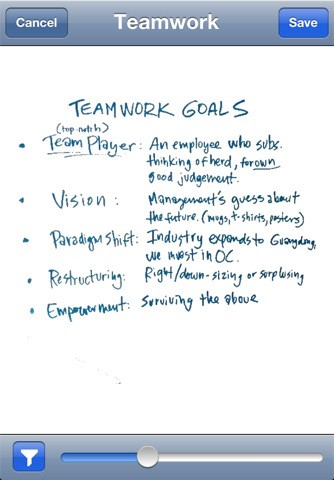
\includegraphics{images/team1.jpg}
			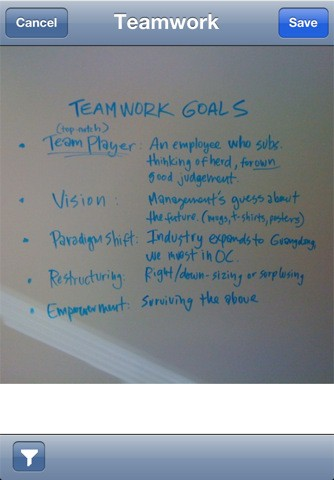
\includegraphics{images/team2.jpg}
			
			Notice the slider at the bottom of the image on the left. This is the contrast slider that helps remove background noise.

			(guesswork)
			Contrast sliders work by analyzing the transition colors between the white and the eventual blue of the writing. The higher the contrast, the faster the transition must be between pure white and pure blue. If the transition is too slow, the transition pixels are assumed to be noise and removed from the photo. This is useful both in making the handwriting appear crisp and in removing random background smudges. Smudges are of course removed because they don’t have the crisp transition periods found in the writing on the board.
			(Now back to research)
			
		\subsection{WBConference}
			This is an Android app that competes with our product because it is another whiteboard capturing device. WBConference differs from Whiteboard Capture Pro in that it is able to automatically recognize which sections of the board are whiteboard. This then allows it to apply its “magnified keystone correction” to remove the excess background imagery. In cases that it cannot recognize the board you can zoom in on just the board boundaries manually before capturing the image. The app has contrast adjustment and image rotation as well so you can take images from any orientation without problems.\\
			
			This app has editing features as well so you can add postscripts or speech bubbles to the images. The files can then be saved as PDFs along with any notes you want to add to them. This app has a widget for the home screen for quick image capturing, and you can set up an email address for quick delivery of the images to an external source.\\

		\subsection{CamScanner -Phone PDF Creator}
			This is the most downloaded 'scanner' app on the market.\\
			
			With it you can take photos of any document, whiteboard, etc that you want. You then go through an editing process in which you can select the important portion of the photograph, change the detail level, contrast, light/darkness etc. It will then save your new document in any number of saved folders. You can make notes about each image and these notes will be saved with the image. You can email, print, fax, or transfer via Bluetooth any of the photos. You can also upload your images to google docs, evernote, skydrive, dropbox, or box.net. \\
			
			These documents get saved as PDFs.\\
			
			There are different enhancement modes: No enhance, low and high enhance, gray mode, and BandW Document modes. These different modes will be better depending on the environment or object that you’re trying to scan. The BandW mode is particularly helpful when scanning books/papers because it does a better job of removing the background noise. \\
			
			CamScanner allows for batch photo taking and batch photo scanning, so you can take multiple pictures and it will scan them all at the same time.\\
			
			You can password protect your documents and even save different document sizes.\\
			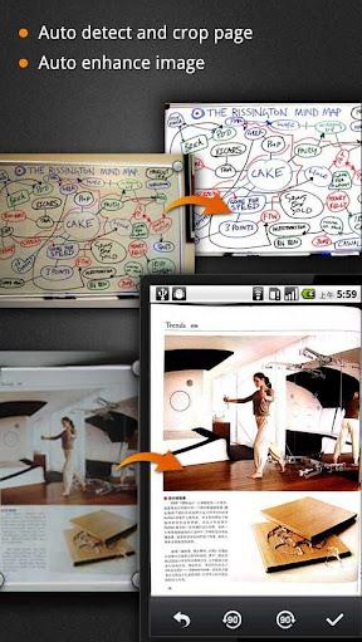
\includegraphics{images/autoCrop.jpg}	

		\subsection{Whiteboard Snap}
		
		This app is a dumbed down version of the previous three. It does the job, it scans and enhances images, it just isn’t as well known as the others and thus doesn’t have the money/time to invest in extra features.\\
		
		This aside, it does work, it is free, and it does save images as PDFs for later use. You can email these photos to yourself and store them in different photos. You can attach notes to your images and you can enhance the quality of the whiteboard picture with their auto-enhance tool.\\
		On the upside, it IS a much smaller program than your avg whiteboard capture app. Over all a smaller lighter free alternative.\\
		I installed this app on my phone and I had trouble using it because it kept crashing.\\

	
	% Fifth Entry
	\section{Group Meeting with Clients 09/12/2012}
		\subsection{Base System Requirements}
			\begin{itemize}
				\item Images must be easy to transfer to the student
					\subitem Could be sent via email, through a link inviting them to view a different site, net space, etc.
				\item Professor must be able to review the images before okay-ing them for distribution.
					\subitem Must be able to select different ‘key’ images if they want.
				\item Must be able to enlarge/interact with and edit after export
				\item System should not need to be plugged in
				\item Set up can be longer the first time as long as you can save the settings so that it doesn’t take so long in the future.
					\subitem Setup vs. Calibration
					\subitem Active time vs inactive time
						\subsubitem It can take longer to set up if it doesn’t need constant attention. Inactive time to set up is much better than active time.
					\subitem 5 min reasonable
				\item Time stamps of when erasing happens
					\subitem Goal 1: End product
					\subitem Goal 2: Step by step board
			\end{itemize}
	
	
	% Fourth Entry
	\section{Individual Work on Further Research and Website Content 09/12/2012}
		\subsection{Website Content}
			\begin{itemize}
				\item Added calendars to both the front page and our meetings page.
				\item Created new ProPANE calendar
				\item Added Griffin's Calendar and ProPANE's calendar to website calendar
			\end{itemize}
		\subsection{Further Research}
			Found a page that seems to have a piece of demo software available to those with access to Microsoft Research’s internal website:\\
			http://research.microsoft.com/en-us/um/people/zhang/WhiteboardIt/\\
			This system takes an image and filters out key information.
			
			The software and technology as a whole is still in its research/development stages. It is a joint project with MS Research and MS Hardware called Distributed Meetings. They have a few technologies going together: A 360 degree video and audio recorder, a Whiteboard image capturing system, (most relevant to us) a PC graphics capture system. Their idea is to record the meeting in several different ways, and then provide easily accessible ways to view all meeting content.
		
			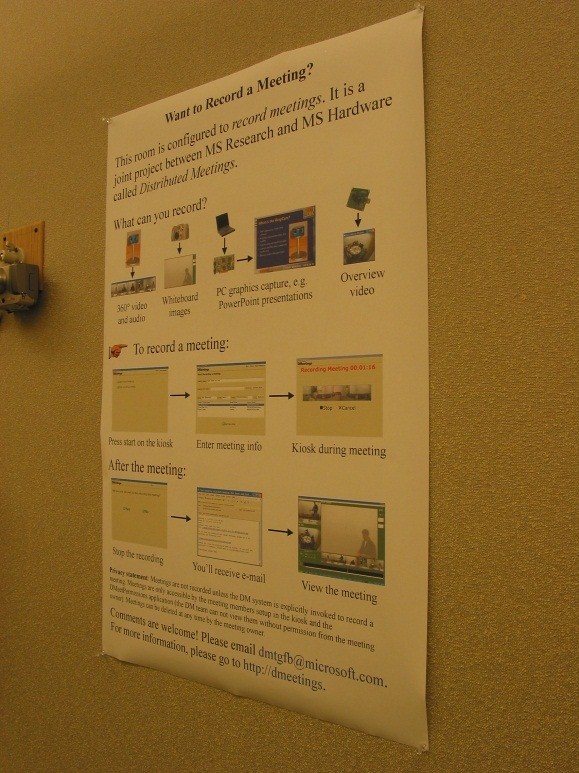
\includegraphics{images/WhiteboardIt.jpg}
			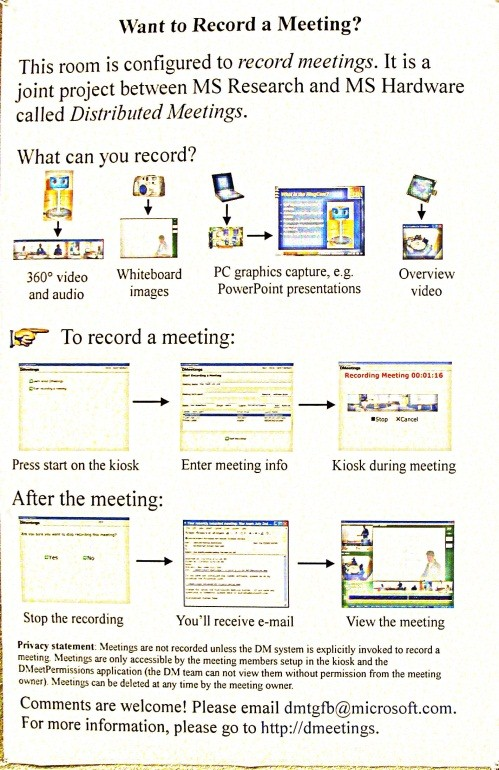
\includegraphics{images/WhiteboardIt2.jpg}\\
			
			We may wish to contact dmtgfb@microsoft.com to ask for more information on their image processing algorithms later on in the process.\\
			\\
			I’m not sure how helpful this might be, but here is a link to Ink-Enabled Apps For Tablet PC\\
			http://msdn.microsoft.com/en-us/magazine/cc967278.aspx\\
			\\
			http://www.fxpal.com/?p=reboard\\
			http://arxiv.org/abs/0911.0039\\
			The following is a paper that talk about another whiteboard captureing technology called ReBoard:\\
			http://arxiv.org/ftp/arxiv/papers/0911/0911.0039.pdf\\
			http://www.fxpal.com/publications/FXPAL-PR-10-546.pdf\\
			
		\subsection{Additional Apps:}
			\begin{itemize}
				\item Whiteboard Capture
				\item Whiteboard Share
				\item WBConference
				\item Whiteboard Snap
				\item BoardTable
			\end{itemize}

	
	% Third Entry
	\section{09/11/2012}
		I first uploaded pictures to the website for our personal biographies.
		\\
		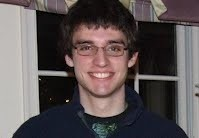
\includegraphics{images/Griffin.jpg}
		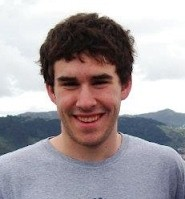
\includegraphics{images/Colin.jpg}
		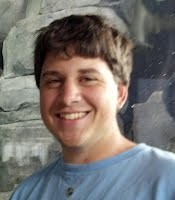
\includegraphics{images/Phil.jpg}
		\\
					After this I wrote an overview about ProPANE on our front page:\\
			Welcome to the website for the Electrical and Computer Engineering senior design project led by Griffin Dunn, Phil Stahlfeld, and Colin Madigan.
			ProPANE's goal is to design and implement a system that will automatically capture all information written on a board during class. This system will then present the saved information in a readily accessible manner so that Bucknell can both better meet the needs of students with disabilities and provide professors with a means to easily compare their notes with the actual information presented in a lecture.
			This project was motivated by Bucknell’s desire to cheaply meet the needs of their students with disabilities. Hiring professional note takers is an expensive endeavor and finding cheaper alternatives is much more desirable.
			This project involves the capture of information from a 2D surface. It will likely require image capture and image processing technology.
		\subsection{Design Constraints}
			\begin{itemize}			
				\item ProPANE must be fully autonomous. After setup the system should require little to no outside interference. The professor should be able to turn it on and leave it running during class and afterwards return to find a set of images depicting everything that was on the board during class.
				\item The information must be presented in a format that allows for easy manipulation, zooming, and editing so that students with disabilities can easily view all content that is displayed on the board.
				\item The system must be discreet. It cannot make loud noises, flashes of light, or create any other forms of distraction during class. Students must be able to concentrate on the lecture not the board capture device.
			\end{itemize}

	
	
	% Second Entry
	\section{Individual Work on Competing Technologies 09/05/2012}
		We have three technologies to compete with: 
		
		\subsection{The Phone App}
			There are several smartphone apps out there that will scan pictures of white boards and filter out the unnecessary information. These applications range from free to a couple dollars on most app stores.\\
				http://www.beetlebugsoftware.com/ is a good example. \\

				Other notable apps:
					\begin{itemize}
						\item Qipit White
						\item Genius Scan
						\item JotNot Scanner Pro
						\item Whiteboard Capture Pro
					\end{itemize}

			However, this IS an issue because it is an area that could possibly pose legal problems. If the resolution is too poor, then the system would be giving ProPANE reliant students a disadvantage. In my opinion, that would be a complete failure of the project.\\
			
		\subsection{Scanners}
			There are scanners that you can attach to an existing white board. After calibrating these scanners, they track your movements using the combination of the sanner and an electronic pen. These electronic pens have replaceable dry erase tips to draw with and replaceable batteries to keep them charged. Some of them require a projector to display background information and others do not.\\

			Examples:
				\begin{itemize}
					\item MimoCapture
					\item eBeam System 3
					\item Interlink FreeBeam
				\end{itemize}

			
		\subsubsection{Electronic Whiteboards}
			Electronic whiteboards are special boards that sense pressure and can display electronic pen interactions with a high degree of accuracy. These displays come in two standard varieties: Those that are electronic displays and those that require a projector to project both the images and any user-inputted writing. Electronic whiteboards tend to be the easiest to use, but they're not very portable because the entire board is required. The trade-off for poor portability is that they can do much more. Multiple people can interact with the board at the same time, and it can be a much more interactive experience. \\

			Examples:
			\begin{itemize}
				\item Smarttech’s SMARTboard 
				\item Panasonic’s Panaboard 
				\item Hitachi’s Starboard 
				\item The Promethean board 
			\end{itemize}

	
	%First Entry
	\section{Initial Group Meeting 08/30/2012}
			\emph{With Phil Stahlfeld and Colin Madigan}\\
			
			Began working on group tasks:
			\begin{itemize}
				\item Team Name
				\item Team Logo
				\item Document Template
				\item Design Specifications
			\end{itemize}
			
		\subsection{Team Name}
			After some discussion we decided that names such as ‘White board scanner’ and ‘board capture system’ weren’t catchy enough. We decided to create an acronym instead so to make our name catchier and thus more memorable. Colin finally came up with our final acronym: ProPANE, short for Professional Portable Automatic Note Extractor. With this agreed upon we moved on to deciding upon our team logo. \\

		\subsection{Team Logo}
			We decided that our logo had to relate to our team name, so with that in mind we searched for images related to the molecular structure of propane. Our favorite image is shown below, and has been adopted as our team logo:\\
			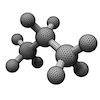
\includegraphics{images/logo.jpeg}\\

		\subsection{Document Template}
			We decided to use LaTEX as our default layout manager for all of our documents. We chose this formatter because it takes care of all the formatting and leaves us with the job of finding and preparing the information, which is the more important part of our job. 

		\subsection{Technical Specifications}
			As noted in our first deliverable, “The goal of this project is to create a system that captures all of the information written on a board during a class in a readily accessible manner. The two driving forces behind solving this problem are: autonomous collection of notes for students with disabilities and providing a means for professors to compare their notes with the actual information presented during a lecture.” \\

			We will be meeting with Robert Midkiff and Douglas Gabauer on 09/13/2013 to discuss more detailed specifications for the project.\\

		
	
	
\end{document}
